\documentclass[10pt,a4paper]{article}
\usepackage[T1]{fontenc}
\usepackage[margin=25mm]{geometry}
\usepackage{amsmath,amssymb,booktabs,graphicx}
\usepackage[nopatch=footnote]{microtype}
\usepackage{xurl}
\usepackage[hidelinks]{hyperref}
% Publication values exported from archived BTS artifacts on 2026-10-13.
% See draft_provenance.json; no new simulations were run.
\newcommand{\BtsPeakX}{31.4368}
\newcommand{\BtsPeakY}{50.7459}
\newcommand{\BtsMedianX}{0.00208629}
\newcommand{\BtsMedianXLo}{0.00207403}
\newcommand{\BtsMedianXHi}{0.00209890}
\newcommand{\BtsDispResidual}{4.382}
\newcommand{\BtsMerit}{1.2906}
\newcommand{\BtsStrengthRows}{%
q11 & +0.448572 & -0.367525 & [-2.5, 2.5] \\
q12 & -1.026778 & -1.216433 & [-3.0, 3.0] \\
q13 & +0.887640 & +1.586072 & [-3.0, 3.0] \\
q21 & -1.066465 & -1.068373 & [-3.0, 3.0] \\
q22 & +1.488384 & +2.823108 & [-3.0, 3.0] \\
q23 & -0.669894 & -2.490968 & [-3.0, 3.0] \\
q31 & +0.589886 & +2.042678 & [-3.0, 3.0] \\
q32 & -1.168702 & -1.434271 & [-3.0, 3.0] \\
q33 & +0.941655 & +0.351115 & [-2.5, 2.5] \\
}
\newcommand{\BtsQuantileRows}{%
$\mathcal M_x$ [1] & 0.002086 & [0.002074, 0.002099] & 0.016482 & 0.028814 \\
$\mathcal M_y$ [1] & 0.002499 & [0.002483, 0.002514] & 0.020701 & 0.035932 \\
$\beta_{x,\max}$ [m] & 31.438418 & [31.430758, 31.445751] & 35.564889 & 37.521376 \\
$\beta_{y,\max}$ [m] & 50.751986 & [50.746458, 50.757604] & 53.831455 & 55.275722 \\
}
\newcommand{\BtsSeedRows}{%
42 & 50,000 & 0 & 0.00210273 & $20.830\times10^{-6}$ & Not met \\
123 & 50,000 & 1 & 0.00207934 & $11.436\times10^{-6}$ & Not met \\
777 & 50,000 & 0 & 0.00210260 & $10.567\times10^{-6}$ & Not met \\
2026 & 400,000 & 4 & 0.00208351 & $2.395\times10^{-6}$ & Met \\
}

% Exported from selected Reviewer 1 numerical results; see final provenance.
\newcommand{\BtsAltPeakX}{33.57950}
\newcommand{\BtsAltPeakY}{28.18004}
\newcommand{\BtsClearMean}{0.01461}
\newcommand{\BtsClearLo}{-0.01791}
\newcommand{\BtsClearHi}{0.04832}
\newcommand{\BtsNomClear}{16.86677}
\newcommand{\BtsAltClear}{16.88139}
\newcommand{\BtsNominalMinimum}{17.45461}
\newcommand{\BtsResponseCondition}{57.78074}
\newcommand{\BtsMachineLossUpper}{1.48670}
\newcommand{\BtsParticleLossUpper}{3.07406}

\title{Supplementary evidence: beta reduction and physical clearance}
\author{Chong Shik Park}
\date{October 13, 2026}
\begin{document}
\maketitle
This supplement preserves the original main-branch campaign. It distinguishes
historical optical statistics from the new particle/clearance comparison.
Original reviewed assets and campaign records remain frozen; historical claims
are interpreted with their original beam and modelling limitations.

\section{Original matching and local response}
The historical three-start replay reproduces one feasible success, one
infeasible success and one budget failure (Table~\ref{tab:starts}). The
successful infeasible candidate illustrates why matching and feasibility are
separate; the failed candidate is not another low-residual match. Three starts
do not establish optimizer reliability, search topology or feasible volume.

\begin{table}[htbp]\centering
\caption{Historical replay outcomes. The initial start is nominal, not random.
J is the scaled residual sum of squares. Feasibility is assessed after search.}\label{tab:starts}
\begin{tabular}{lrrrr}\toprule
Start & J & peak $\beta_x$ [m] & peak $\beta_y$ [m] & outcome\\\midrule
Nominal & $1.29\times10^{-13}$ & 31.437 & 50.746 & feasible success\\
Random 1 & $1.21\times10^{-12}$ & 25.329 & 62.556 & infeasible success\\
Random 2 & 1284.86 & 69.921 & 65.043 & budget failure\\
\bottomrule\end{tabular}\end{table}

The archived raw/rounded strengths remain feasible at 40-step resolution and
independent-map precision. Table~\ref{tab:strengths} supplies numerical values;
decimal digits do not prescribe power-supply accuracy. Optical functions,
dispersion and projected RMS sizes appear in Fig.~\ref{fig:optics}. Beta peaks
reported here are element-boundary samples rather than continuous maxima.

\begin{table}[htbp]\centering
\caption{Reference and alternative settings [m$^{-2}$], with reference gradient
[T/m] and assumed-bore pole field [T]. Negative K indicates defocusing in x.}\label{tab:strengths}
\begin{tabular}{lrrrr}\toprule
Quad & Reference K & Alternative K & Reference G & $|B_{\mathrm{pole}}|$\\\midrule
q11 & -0.367525 & 0.060274 & -4.904 & 0.095 \\
q12 & -1.216433 & -2.126974 & -16.230 & 0.314 \\
q13 & 1.586072 & 1.869755 & 21.162 & 0.409 \\
q21 & -1.068373 & 0.954499 & -14.255 & 0.276 \\
q22 & 2.823108 & -0.258649 & 37.667 & 0.729 \\
q23 & -2.490968 & -1.197779 & -33.236 & 0.643 \\
q31 & 2.042678 & 2.817163 & 27.255 & 0.527 \\
q32 & -1.434271 & -3.000000 & -19.137 & 0.370 \\
q33 & 0.351115 & 0.901619 & 4.685 & 0.091 \\
\bottomrule\end{tabular}\end{table}

\begin{figure}[htbp]\centering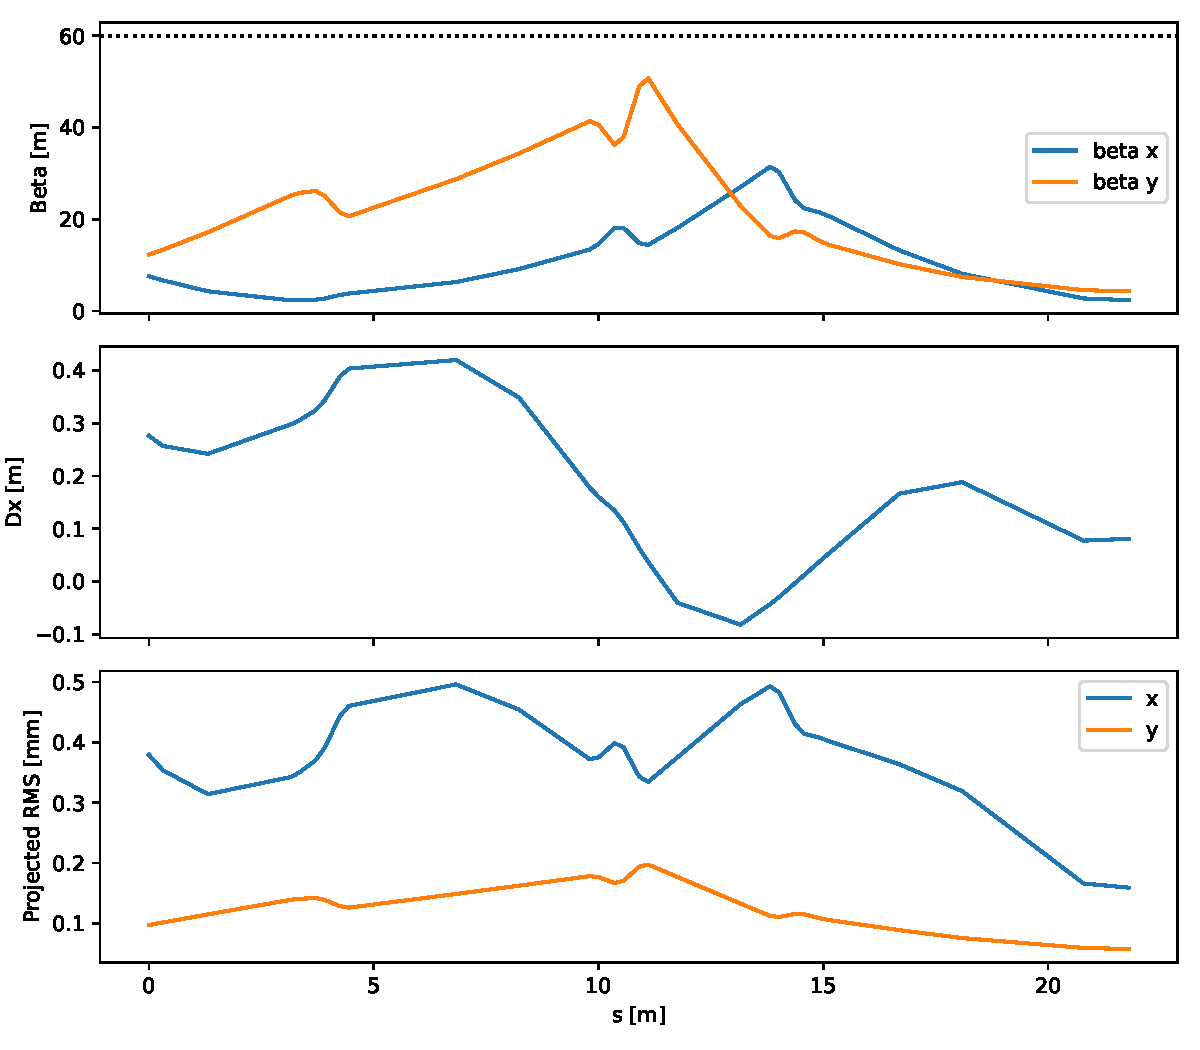
\includegraphics[width=.85\linewidth]{figures/optics.pdf}
\caption{Reference element-boundary beta, horizontal dispersion and projected
RMS sizes for the design beam. The dotted beta line is the assumed optical
screening ceiling, not a vacuum-chamber edge.}\label{fig:optics}\end{figure}

For local sensitivity diagnostics we normalize rows by the optical scales and
columns by an assumed common $0.01$ m$^{-2}$ tuning increment:
$A_{ij}=(\partial O_i/\partial K_j)\Delta K_j/\sigma_i$.
Central steps $10^{-4},10^{-5},10^{-6}$ m$^{-2}$ converge; the six active modes
and three-dimensional local null space have condition number
\BtsResponseCondition. Six finite small-mode perturbations remain inside bounds
and agree with linear predictions within 1\%. This differs from the archived
mixed-unit condition number 1421.636. Neither Euclidean singular-vector
orthogonality nor a local null space guarantees finite optical decoupling.
Achieved commissioning correction claims are withdrawn: measurements, actuator
calibration and estimation uncertainty have not been established.

\section{Historical optical statistics}
Reconstruction of all 550,000 historical observations confirms five optical-rule
exceedances, no invalid evaluations, and compatible model/target/error inputs
across four runs. The rule is $\beta_{x,\max}$ or $\beta_{y,\max}>60.01$ m,
or $\mathcal M_x+\mathcal M_y>2.05$, where
$\mathcal M_u=\tfrac12\mathrm{Tr}(\Sigma_{u,t}^{-1}\Sigma_{u,o})-1$
uses unit-emittance transverse matrices. All five failures exceed vertical beta
only (60.23--61.64 m); they are not physical losses.

The descriptive optical-failure estimate is $5/550000=9.09\times10^{-6}$ with
exact asymmetric 95\% limits $[2.95\times10^{-6},2.12\times10^{-5}]$; Wilson
limits are $[3.8831\times10^{-6},2.1283\times10^{-5}]$~\cite{Wilson1927,Clopper1934}.
The pooled horizontal median \BtsMedianX\ has the order-statistic interval
[\BtsMedianXLo, \BtsMedianXHi], not a pooled-bootstrap interval. Reconstructed
median, 95th and 99th quantile intervals match the archived analysis.

Three 50,000-sample median-prefix changes (20.830, 11.436 and
10.567)$\times10^{-6}$ miss the $10^{-5}$ target; the 400,000 follow-up
change $2.395\times10^{-6}$ passes. This is median stability, not rare-tail
convergence. The follow-up stopping decision is not archived as predeclared;
fixed-N intervals do not certify sequential coverage. Historical one-at-a-time
sensitivity is mean absolute change of $\mathcal M_x+\mathcal M_y$, not J.
Seed42 ranks beta-only entrance errors (0.00890374), gradients (0.000861122)
and energy (0.000106336). Near-zero alignment/roll mismatch does not certify
alignment/coupling tolerances. Historical and new-model data remain separate.

\section{Finite loss events and numerical validation}
The new inference export contains exact block binomial intervals and independent
reconstruction of all nine paired clearance intervals. Zero losses among 200
independent three-shot blocks gives one-sided 95\% upper event probability
$1-0.05^{1/200}=0.014867$. A two-sided descriptive binomial calculation for zero
losses among 1.2 million particles gives upper probability $3.0741\times10^{-6}$;
this requires an independence assumption not justified as unconditional machine
reliability. Exact-binomial attribution is Clopper and Pearson~\cite{Clopper1934}.

The complete source-labelled covariance, linearization about actual shot
centroids, uncensored nonlinear Gaussian quadrature, integration/probe convergence
and spatial meshes are available in the attachment. Quadrature certifies moments
only on checked cases, not rare-tail loss probabilities. Comparison retains
first-loss elements, coupled covariance and exact random seeds. Station
transmission ends at m4; unknown continuous chamber and ring capture remain
outside the model.

The initial shared-aperture hypothetical run is excluded and retained with exact
generating sources. The corrected driver independently detaches the selected
station, verified by a regression test. No numerical failure record is silently
counted as physical success.

\bibliographystyle{unsrt}
\bibliography{paper}
\end{document}
